% This is "sig-alternate.tex" V1.9 April 2009
% This file should be compiled with V2.4 of "sig-alternate.cls" April 2009
%
% This example file demonstrates the use of the 'sig-alternate.cls'
% V2.4 LaTeX2e document class file. It is for those submitting
% articles to ACM Conference Proceedings WHO DO NOT WISH TO
% STRICTLY ADHERE TO THE SIGS (PUBS-BOARD-ENDORSED) STYLE.
% The 'sig-alternate.cls' file will produce a similar-looking,
% albeit, 'tighter' paper resulting in, invariably, fewer pages.
%
% ----------------------------------------------------------------------------------------------------------------
% This .tex file (and associated .cls V2.4) produces:
%       1) The Permission Statement
%       2) The Conference (location) Info information
%       3) The Copyright Line with ACM data
%       4) NO page numbers
%
% as against the acm_proc_article-sp.cls file which
% DOES NOT produce 1) thru' 3) above.
%
% Using 'sig-alternate.cls' you have control, however, from within
% the source .tex file, over both the CopyrightYear
% (defaulted to 200X) and the ACM Copyright Data
% (defaulted to X-XXXXX-XX-X/XX/XX).
% e.g.
% \CopyrightYear{2007} will cause 2007 to appear in the copyright line.
% \crdata{0-12345-67-8/90/12} will cause 0-12345-67-8/90/12 to appear in the copyright line.
%
% ---------------------------------------------------------------------------------------------------------------
% This .tex source is an example which *does* use
% the .bib file (from which the .bbl file % is produced).
% REMEMBER HOWEVER: After having produced the .bbl file,
% and prior to final submission, you *NEED* to 'insert'
% your .bbl file into your source .tex file so as to provide
% ONE 'self-contained' source file.
%
% ================= IF YOU HAVE QUESTIONS =======================
% Questions regarding the SIGS styles, SIGS policies and
% procedures, Conferences etc. should be sent to
% Adrienne Griscti (griscti@acm.org)
%
% Technical questions _only_ to
% Gerald Murray (murray@hq.acm.org)
% ===============================================================
%
% For tracking purposes - this is V1.9 - April 2009

\documentclass{acm_proc_article-sp}
\usepackage{graphicx}
\usepackage{subfigure}
\usepackage{wrapfig}

\begin{document}
%
% --- Author Metadata here ---
%\conferenceinfo{ARM}{'97 El Paso, Texas USA}
%\CopyrightYear{2007} % Allows default copyright year (20XX) to be over-ridden - IF NEED BE.
%\crdata{0-12345-67-8/90/01}  % Allows default copyright data (0-89791-88-6/97/05) to be over-ridden - IF NEED BE.
% --- End of Author Metadata ---

\title{Reusing Legacy Software in a Self-adaptive Middleware Framework}
%\subtitle{[An Evaluation of OSGi]}
%\titlenote{A full version of this paper is available as
%\textit{Author's Guide to Preparing ACM SIG Proceedings Using
%\LaTeX$2_\epsilon$\ and BibTeX} at
%\texttt{www.acm.org/eaddress.htm}}}

%
% You need the command \numberofauthors to handle the 'placement
% and alignment' of the authors beneath the title.
%
% For aesthetic reasons, we recommend 'three authors at a time'
% i.e. three 'name/affiliation blocks' be placed beneath the title.
%
% NOTE: You are NOT restricted in how many 'rows' of
% "name/affiliations" may appear. We just ask that you restrict
% the number of 'columns' to three.
%
% Because of the available 'opening page real-estate'
% we ask you to refrain from putting more than six authors
% (two rows with three columns) beneath the article title.
% More than six makes the first-page appear very cluttered indeed.
%
% Use the \alignauthor commands to handle the names
% and affiliations for an 'aesthetic maximum' of six authors.
% Add names, affiliations, addresses for
% the seventh etc. author(s) as the argument for the
% \additionalauthors command.
% These 'additional authors' will be output/set for you
% without further effort on your part as the last section in
% the body of your article BEFORE References or any Appendices.

\numberofauthors{3} 

% 4th. author
%\alignauthor Sabine Moisan\\
%       \affaddr{INRIA Sophia-Antipolis}\\
%       \affaddr{2004 Route des Lucioles, BP 93}\\
%       \email{Sabine.Moisan@inria.fr}
% 5th. author
%\alignauthor Jean-Pault Rigault\\
%      \affaddr{INRIA Sophia-Antipolis}\\
%       \affaddr{2004 Route des Lucioles, BP 93}\\
%       \email{jpr@unice.fr}

\author{
\alignauthor
Santiago Hurtado\\
       \affaddr{Universidad de los Andes}\\
       \affaddr{Bogota, Colombia}\\
       \email{s-hurtad@uniandes.edu.co}\\
% 2nd. author
\alignauthor
Sagar Sen\\
       \affaddr{ATLANMOD, Ecole des Mines}\\
       \affaddr{Nantes, France}\\
       \email{sagar.sen@mines-nantes.fr}\\
% 3rd. author
\alignauthor Rubby Casallas\\
        \affaddr{Universidad de los Andes}\\
       \affaddr{Bogota, Colombia}\\
       \email{rcasalla@uniandes.edu.co}\\ 
}


\maketitle
\begin{abstract}
Software that adapts its behavior to an operational context and/or feedback from within is self-adaptive. For instance, a computer vision system to detect people may change its behavior due to change in context such as nightfall. This may entail automatic change in architecture, software components and their parameters at runtime. Legacy software components do not possess this ability. Therefore we ask, can legacy software be successfully cast into a self-adaptive middleware framework ?  We present Tekio, a self-adaptive middleware platform to dynamically compose legacy software behavior. Tekio is based on \emph{dynamic component loading} available in a Java implementation of Open Service Gateway Interface (OSGi). Tekio contains generic components to capture context/feedback, plan an adaptation strategy, and reconfigure domain-specific components. The domain-specific components encapsulate legacy behavior implemented possibly in native languages such as C/C++. We implement a self-adaptive vision system in Tekio as a case study. We perform experiments to validate that the self-adaptive layer based on OSGi has negligible effects on the performance of the legacy software. We also demonstrate that the self-adaptive middleware can handle about 30 adaptations in a span of 2 seconds while producing meaningful output.
\end{abstract}

% A category with the (minimum) three required fields
%\category{H.4}{Information Systems Applications}{Miscellaneous}
%A category including the fourth, optional field follows...
%\category{D.2.8}{Software Engineering}{Metrics}[complexity measures, performance measures]


\keywords{Self-adaptive software, OSGi, legacy software, software reuse}

%-------------------------------------------------------------------------------------------------------------------
\section{Introduction}
\label{sec:introduction}

Self-adaptive systems dynamically modify themselves due to contextual changes and feedback from within their own components \cite{Oreizy}. Contextual changes may emanate from monitoring events from the physical environment, running software/hardware components, and detectors of social and lingual boundaries to name a few. Moreover, these software systems continue running  despite user interventions and failures in the underlying software and hardware \cite{Brun2009}. Well known examples of such systems are sites such as Facebook and Google.  Contrary to these modern systems legacy software systems/libraries were not built with continual execution, adaptation to context and fault tolerance in mind. Therefore, a natural question arises: Can we reuse existing legacy libraries as components in a self-adaptive framework where they can be loaded/unloaded/replaced at runtime?

Reusing legacy libraries in a self-adaptive middleware framework is the subject of this paper. Legacy libraries are often available in the form of \emph{compiled objects}. These objects are typically black-boxes with callable functions. For instance, the  computer vision library OpenCV \cite{Zelinsky2009} contains functions to segment images and detect different types of objects. Different legacy libraries may be available in many different programming languages. In a typical native implementation, these legacy functions are sequentially called in a static program, that is first compiled and then executed with core behavior that is practically immutable at runtime.   Our target self-adaptive middleware framework aims to create self-adaptive systems using legacy libraries whose behavior can change at runtime. We aim to (a) separate legacy library functionality into components (b) achieve interoperability between components in different languages (c) automatically (re)configure a set of components in a processing chain based on contextual events and feedback events from the system itself (d) monitor Quality of Service (QoS) and evaluate system performance.

In this paper, we present the self-adaptive middleware framework, Tekio. Tekio adheres to the requirements in  \cite{Hallsteinsen2006} for component frameworks to implement dynamic self-adaptive systems. It has the following functionality:(1) Component management that helps define components and the interactions amongst them called a system configuration, (2) Instance management that permits the component life-cycle to be administered and (3)Self-adaptation management for context understanding and mapping context to a system configuration. Tekio is a implemented in Java and provides access to legacy libraries in different languages via Java Native Access (JNA). Self-adaptation in Tekio is achieved using \emph{dynamic component loading}  provided by the  OSGi framework specification (formerly known as the Open Services Gateway Initiative). OSGi provides an universal publish-subscribe based protocol for components with different underlying implementation languages to communicate with each other. The OSGi framework has applications ranging from mobile applications, IDE, applications servers to software in automobile industries. The OSGi has 136 official members plus several research projects. It has seven implementations such as Eclipse Equinox, Apache felix, Knopflerfish and projects such as JBoss, Glasfish Fuse EXB Eclipse platform and WebSphere. The widely used OSGi provides the basic functionality to create self-adaptive systems. This paper serves as an evaluation of OSGi to realize self-adaptive middleware and systems.

We use Tekio to build a self-adaptive vision system. This system serves as a case study to evaluate Tekio and OSGi as the middleware framework to reuse legacy open-source libraries. We reuse the OpenCV libraries \cite{Zelinsky2009} in software components dynamically managed by Tekio. Tekio components call native code in C/C++ using Java Native Access. We provide number of configurations of these components for adaptation. These configurations achieve tasks such as intrusion detection, face detection, and segmentation. During adaptations we measure frames per second indicating throughput. We also measure the settling time between adaptations. Settling time indicates the time required by Tekio to produce meaningful outputs after adaptation. We perform experiments to demonstrate that Tekio's throughput for a configuration is very close to an identical native implementation despite the layer of software for self-adaptation. The self-adaptive system can demonstrate very low settling times for low and medium resolution input video. For instance, it can provide about 30 adaptations in a span of 2 seconds without significant loss in throughput. However, for high resolution input videos the system cannot adapt is allowed to adapt less frequently to provide meaningful outputs. From these results we incur that managing  self-adaptation requires rigorous empirical analysis and may entail trade-offs.

The paper is organized as follows.  In Section \ref{sec:architecture}, we present Tekio's architecture based on OSGi. In Section \ref{sec:validation}, we validate Tekio. In Section \ref{sec:relatedwork}, we present the comparison of Tekio with other self-adaptive middleware frameworks. We conclude in Section \ref{sec:conclusion}.



\section{Architecture}
\label{sec:architecture}

In this Section, we present the \emph{Self-Adaptive Middleware} called \emph{Tekio}.  The middleware framework allows arrangement of  legacy modules in a processing chain that is self-adaptive. Tekio is a component centric architecture  that provides possibility to replace any of its components at runtime and maintain a clear separation of concerns that is between self-adaptation and behavioral components. Tekio is built in layers as shown in Figure \ref{fig:tekioArch} (a). The lowest software layer is that of OSGi including the Java Virtual Machine. The OSGi layer is primarily responsible for execution of the system using the publish-subscribe paradigm for service oriented architecture. The legacy libraries are called from within domain-specific OSGi components in the second layer. The Java Native Access library is used to access the native library. Finally, Tekio's self-adaptation components (see Section \ref{sec:sec:selfTekio}) manage these domain-specific OSGi components (see \ref{sec:sec:chainTekio}). 

% Put the images side by side.


\begin{figure}
%	[H] \centering 
	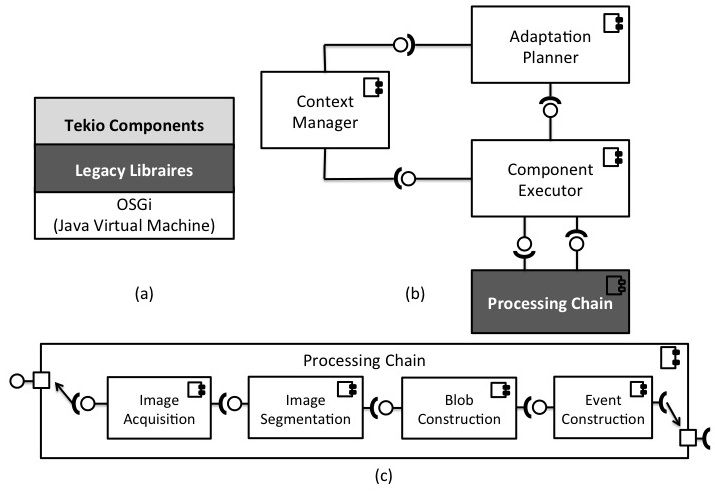
\includegraphics[scale=0.3]{images/architecture.jpg}
	 \caption{Tekio (a) Software Layers (b) Generic Architecture (b) Domain-specific Architecture}
	 \label{fig:tekioArch} 
\end{figure}

\subsection{Tekio Self-adaptation Components} 
\label{sec:sec:selfTekio}

Tekio's self-adaptation is provided by three components as shown in Figure \ref{fig:tekioArch} (b):  (1) The Context Manager that monitors and analyzes context events to know when to request a change in processing chain configuration (2) The Adaptation Planner that produces a change plan and (3) The Executor component that (re)configures the processing chain  and executes it. The new processing chain itself can produce new feedback contextual events. The methodology is based on  the Monitor, Analyze, Plan, Execute, Knowledge (MAPE-K) conceived by IBM in \cite{IBM2005}. At this moment the system is capable of self-configuring and self-optimizing based on QoS feedback and context awareness. 

Tekio is able to provide four different adaptations types: (a)Parameter Adaptation of any of the running components, (b) Component Adaptation to replace a component at runtime for another that provides a similar task, (c) Context Event Adaptation, depending on events from the  processing chain the system analyzes how to adapt and request a new adaptation, and (d) QoS Adaptation on which the system is able to maintain a minimum level of quality of service. 

\subsection{Processing Chain}
\label{sec:sec:chainTekio}

A processing chain as shown in Figure \ref{fig:tekioArch} (c)  is the current configuration of domains-specific components managed by Tekio. We implement a self-adaptive vision system using Tekio. The domain-specific/vision OSGi components in the processing chain call algorithms implemented in the open-source computer vision library OpenCV(Open Source Computer Vision) 2.1. This library is written in C and C++, as many other computer vision libraries for performance benefits. 

We achieve the link between OSGi and legacy libraries using the Java library, Java Native Access (JNA), that seamlessly calls C/C++ functions with negligible performance loss. 
A similar implementation  JavaCV \cite{javacv} uses the native access functionality. Technically,  we pass the memory address of an image to the OpenCV C++ functions. This allows  the OSGi framework to manage the native implementation and its process without compromising its performance and original OpenCV library functionalities. The interfaces of the different algorithms are defined in Java while the implementations of the component is in C++. This improves portability and usability of the vision components with  all other components written in the OSGi framework. Any other OSGi component can execute the functionality of these vision components without worrying about low-level and native implementation detail in C/C++.

The vision system's processing chain consists on four types of algorithms: 1) Image acquisition that provides images from different possible sources such as, cameras, streams or files, 2)Image Segmentation that divides images and extracts important objects, 3) Blob Construction and Object Detection that merges the separate objects  into a group called a blob and then into an object such as a face 4) Event  Construction that converts information at different stages of the vision system to produce either events that are fed back to Tekio or events to final users. Each type of algorithm has several possible implementations that are  different manners or configurations to provide specific tasks. For instance, if we use the Smooth Segmentation and the Find Contours blob construction algorithms the system can detect motion. If the Pyramid Segmentation and the HAAR blob construction algorithms are used the system can detect faces. However, if the last configuration uses FGD Segmentation algorithm instead of the pyramid the system can perform faster FPS but lower result quality.

\subsection{Example Execution in Tekio}

We demonstrate dynamic adaptation in Tekio using  Figure
\ref{fig:exampleExecution}. Tekio starts in intrusion detection mode
which is the initial and current configuration. An intrusion event is
detected as shown in Figure \ref{fig:intrusionDetection} by the context manager. The adaptation planner then decides the new
  configuration for face detection. The component executor loads the face detection component. The face detection configuration ensues as
  shown in Figure  \ref{fig:faceDetection}.


\begin{figure}
\centering
\subfigure[Intrusion Detection]{
	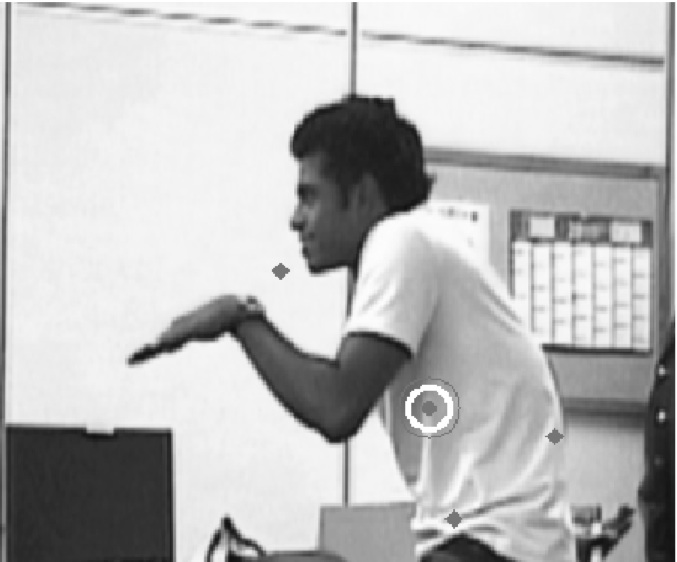
\includegraphics[width=0.3\textwidth]{images/intrusion_detection.jpg}
	\label{fig:intrusionDetection}
}
\subfigure[Face Detection]{
	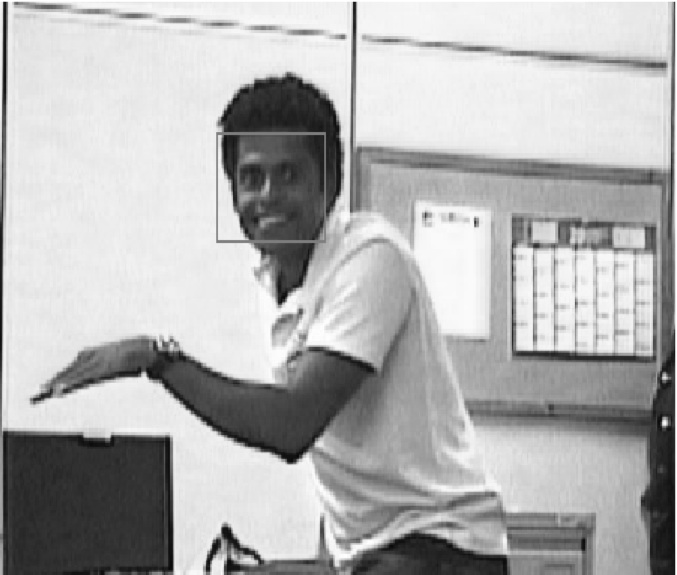
\includegraphics[width=0.3\textwidth]{images/face_detection.jpg}
	\label{fig:faceDetection}
}	
	\label{fig:exampleExecution}
	\caption[Dynamic Reconfiguration from Intrusion to Face Detection]{Dynamic Reconfiguration from Intrusion to Face Detection. Figure \subref{fig:intrusionDetection} is before and Figure \subref{fig:faceDetection} is after}
\end{figure}


\section{Validation}
\label{sec:validation}

Our objective is to validate the self-adaptive middleware Tekio built using an OSGi component framework. The validation aims to encourage the reuse of legacy components in modern self-adaptive frameworks. Our case study is a self-adaptive computer vision system built using Tekio. We choose the representative computer vision domain for a number of reasons: (a) they process large amounts of input data with variations in resolution and content of images, (b) they often require high-throughput and low latency and can run on various operating platforms, (c) they solicit the use of hardware resources such as cameras, high-end  servers, and actuators, and (d) computer vision applications require complex software components involving large databases, file systems, and image processing algorithms.

We are intrigued by two principal questions that we address experimentally:
\noindent \textbf{Q1}:How much performance is compromised due to the use of self-adaptive middleware on a native implementation?
\noindent \textbf{Q2}:How often the system can adapt while maintaining a minimal QoS?

The experimental setup to answer these questions is presented in Section \ref{sec:sec:experimentalsetup}. Finally, we present results of our experiments and discuss them in Section \ref{sec:sec:resultsdiscussion}.


\subsection{Experimental Setup}
\label{sec:sec:experimentalsetup}

Dynamic adaptation is between different system configurations of video processing components handled by Tekio. A configuration is a specific set of components and its parameters. The components in the configuration are composed in a video processing chain/pipeline. In our experiments we implement a total of six configurations in Figure \ref{fig:configurations}.

\begin{figure*}[bht]
   %\fbox{
 %\vspace{-20pt}
 \centering
 \hbox{\begin{minipage}[c]{0.4\textwidth}
       Configurations\\
		\begin{tabular}{ll}
			\hline
	       Number & Name \\ \hline
	       \textbf{C1} & SMOOTH\_SEGMENTATION \\
	       \textbf{C2} & FGD\_SEGMENTATION \\
	       \textbf{C3} & PYRAMID\_SEGMENTATION \\
	       \textbf{C4} & INTRUSION\_DETECTION \\
	       \textbf{C5} & FACE\_DETECTION \\
	       \textbf{C6} & FACE\_DETECTION\_FGD \\ \hline
	       \end{tabular}
   \end{minipage}
	
   \begin{minipage}[c]{0.6\textwidth}
       \begin{center}
	   Configurations Details
       \begin{tabular}{lllllll}
		\hline
       Component & C1 & C2 & C3 & C4 & C5 & C6\\ \hline
       OpenCV AVI Reader &  1 & 1 & 1 & 1 & 1 & 1\\
       Image Smoothing &  2 & $\times$ & $\times$ & 2 & $\times$ & $\times$ \\
       FGD Background Subtraction & $\times$ & 2 & $\times$ & $\times$ & $\times$ & 2\\
       Pyramid Segmentation &  $\times$ & $\times$ & 3 & $\times$ & 2 & $\times$\\
       HAAR Detection &  $\times$ & $\times$ & $\times$ & 3 & 3 & 3\\
       Image Window &  3 & 3 & 4 & 4 & 4 & 4 \\ \hline
       \end{tabular}
       \end{center}
   \end{minipage}}
  % \vspace{-30pt}
  %}
 \caption{Experimental Configurations}
  \label{fig:configurations}
\end{figure*}

%\begin{figure}
%	[H] \centering 
%	\includegraphics[scale=0.5]{images/SystemConfigurations.jpg} \caption{System Configurations} \label{fig:SystemConfigurations} 
%\end{figure}

We present the content of these configurations in Figure \ref{fig:configurations}. For example, the configuration for motion detection contains three different components (a) image acquisition that reads a video from a file, (b) image segmentation that reduces or smoothens the edges of the images, (c) blob construction  that finds the contours of objects and translates them into detected movement. 

Another dimension of variability in our experiments is the image resolution. The input to the video processing chain is 1020 frames of video in an office space available in three different resolutions:1) High, 1024x720 pixels with a bit rate of 3,582 2) Medium, 720x400 pixels with a bit rate of 1,325 and, 3) Low, 480x272 pixels with a bit rate 681. Each experiment measures percentage of CPU usage, percentage of memory usage and FPS monitored every 5 frames. 

We evaluate the configurations based on the following metrics:
	\begin{description}
		\item[Throughput] We measure throughput using the rate at which the video processing chain processes frames per second (FPS).
		\item[Settling Time] The time the system takes to switch from the current configuration to the next. This measurement takes into account the time needed to load the new components
		\item[CPU Usage] What percentage of the processor Tekio is using at a given instant. This includes the percentage of processor used by the loaded vision components.
		\item[Memory Usage] What quantity of memory Tekio is using at any given instant. This measurement also includes includes memory used by vision components in Tekio.
	\end{description}

We design two experiments to address questions \textbf{Q1} and \textbf{Q2}:

\begin{description}	
		\item[Experiment E1] For \textbf{Q1}, we run a single configuration with three resolutions. Each system configuration is first run  with legacy static C components. Second, we run the configuration using  Tekio that handles the C components in its self-adaptive framework. The goal is to understand how much performance is lost by adding the self-adaptive layer, and whether this performance loss out costs the benefits of self-adaptation.
		
		\item[Experiment E2] For \textbf{Q2}, we run 38 pairs (without repetition) of the 6 configurations in a fixed time. First, we reconfigure 38 times in two minutes.	Secondly, we  decrease the time limit to 90 seconds and continue reducing to 60, 45, 30, 15, 10, 5, 4, 3, 2, 1 second(s). The purpose here is to figure how the system is affected by the stress to adapt quickly in fixed time. Can we determine when the system stops functioning properly due to a very high frequency of adaptation?
		
	\end{description}
	
All experiments to answer our empirical questions  are executed on an iMac with the Intel Core i3 Processor of 3.06GHz and 4GB 1333 MHz DDR3.
	
\subsection{Results and Discussion}
\label{sec:sec:resultsdiscussion}

We summarize the results of executing experiment \textbf{E1} in Figure \ref{fig:performanceComparison} and  \textbf{E2} in Figure \ref{fig:stressTesting}.
	%graphs
	\begin{figure*}
	\centering %1415 × 415
		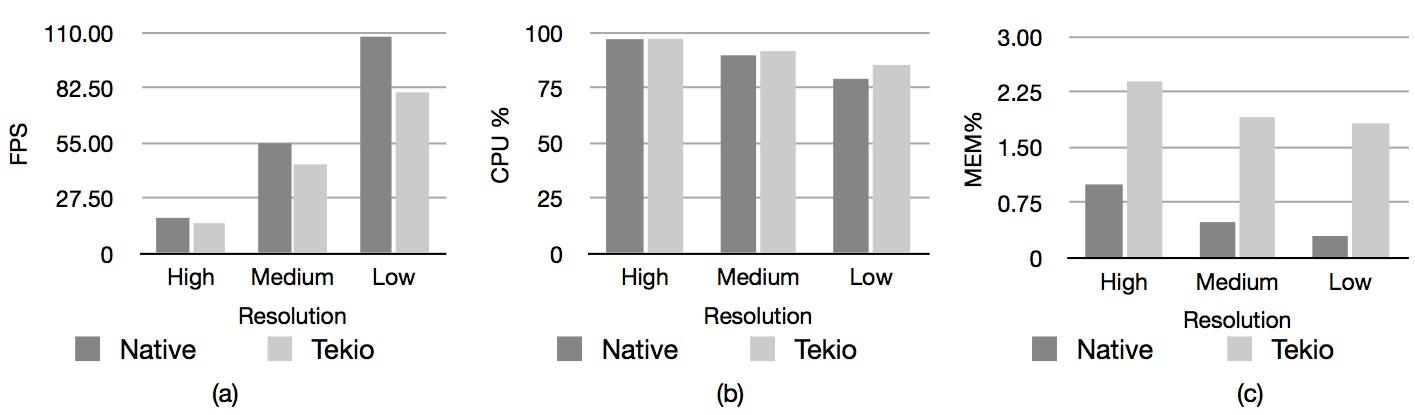
\includegraphics[scale=0.55]{images/MotionDetectionComparison.jpg} 
		\caption{Performance Comparison of Legacy and Self-adaptive for Motion Detection (a) Frame Rate (b) CPU Usage (c) Memory Usage }
		 \label{fig:performanceComparison} 
	\end{figure*}
	
	\begin{figure*}
	\centering 
		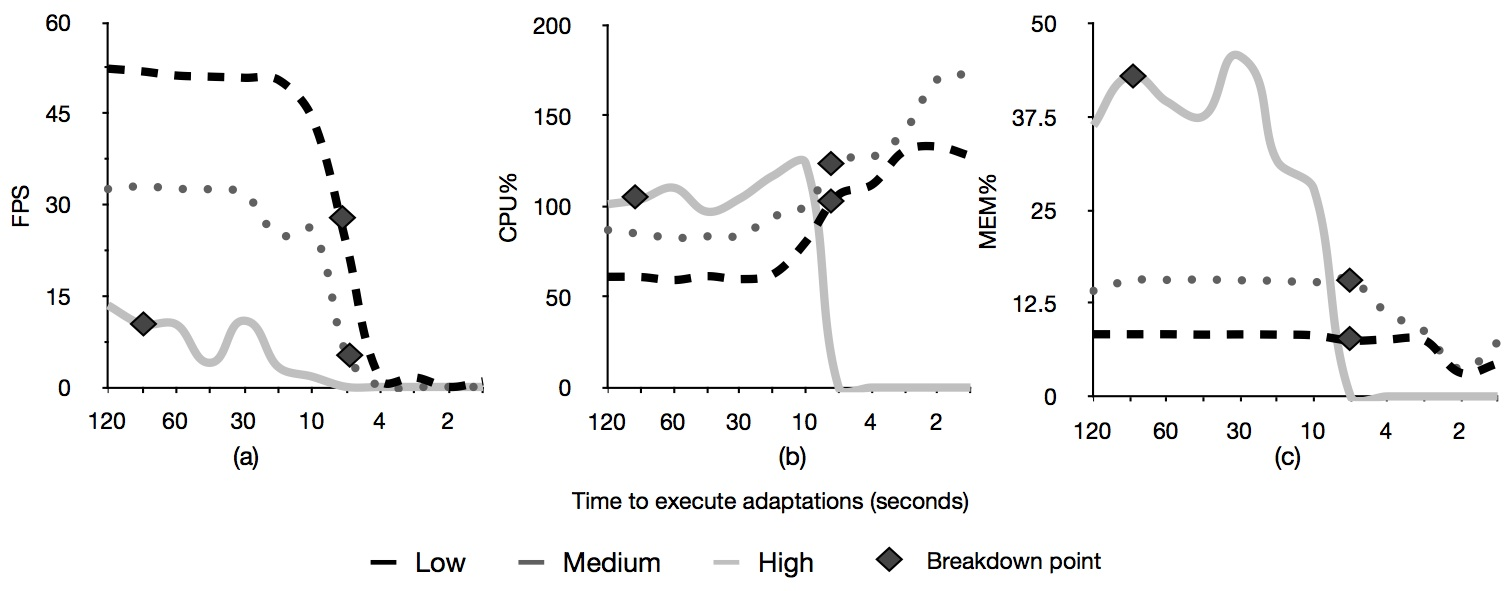
\includegraphics[scale=0.55]{images/StressTesting.jpg}
		 \caption{Stress Testing All Switches to Motion Detection (a) Frame Rate (b) CPU Usage (c) Memory Usage}
		 \label{fig:stressTesting} 
	\end{figure*}
	%How question where answer


In this section, we summarize and present the results of the experimental executions. 


We execute  \textbf{Experiment E1} to address \textbf{Question Q1}. In Figure \ref{fig:performanceComparison}, we compare a legacy  implementation of motion detection in C with motion detection within the self-adaptive framework Tekio. As expected, in Figure \ref{fig:performanceComparison} (a) we observe that the frame rate is \emph{slightly higher} for a native/legacy implementation of motion detection compared to Tekio for all three resolutions low, medium, and high. The CPU usage for both native and Tekio is similar as shown in Figure \ref{fig:performanceComparison} (b). However, we observe large difference in memory usage in Tekio compared to a native implementation as seen in Figure \ref{fig:performanceComparison} (c). The OSGi framework used to develop Tekio uses up considerable amount of memory compared to the native implementation. However, the upper limit is around 2.25\% of main memory (4Gb) which is largely acceptable. 

We execute \textbf{Experiment E2} to address \textbf{Question Q2}. We switch between pairs of configuration using Tekio. In all possible 38 pairs of configurations we choose to show 6 pairs where we switch to motion detection from any given configuration with varying time limits and resolutions. The results for low, medium, and high resolution input videos are are shown in Figure \ref{fig:stressTesting}. In  Figure \ref{fig:stressTesting} (a), we observe that frame rate starts dropping at 90 seconds time bound for high resolution while 5 seconds time bound for low and medium resolution videos. This implies that a high frequency of adaptation is not suitable for high resolution images while we may expect to adapt several times for lower resolution videos. The CPU usage drops for high resolution after its break point as seen in Figure \ref{fig:performanceComparison} (b). However, as the frequency of adaptation increases for low and medium the CPU usage increases beyond using a single CPU (upto 170\%). Finally,  in Figure \ref{fig:performanceComparison} (c), we notice that memory usage for high resolution is initially very high but gradually drops after the break point. The memory usage remains relatively static for low and medium resolution but drops after the break point. 

We define the time required for the system to settle down into a state which produces meaningful results as settling time. In conclusion, we observe that most of the \emph{settling times} are very low. However,  if the system adapts very fast (about 0.25 milliseconds per adaptation) the system can begin to fail depending on the load and video resolution. However, most importantly Tekio does not crash, it simply does not produce results and continues running, this is possible because the algorithms do not produce any exceptions. In future work, we would like to see if Tekio can recover from bursts of high loads automatically without crashing.

\section{Related Work}
\label{sec:relatedwork}

Self-adaptive middleware frameworks are an emerging area in software engineering. There are a number of contributions in the domain self-adaptive middleware. Most self-adaptive middleware are based on the MAPE-K loop proposed by IBM \cite{IBM2005}. An ampl survey is provided in \cite{villegas2011}. We discuss middleware frameworks that are closely related to Tekio. We place our contribution with respect to established frameworks such as WildCAT \cite{David2005}, Rainbow \cite{garlan2004}, DIVA \cite{Romero2010} and MUSIC \cite{Rouvoy2008}.

WildCAT \cite{David2005} is an easy to use Java based framework to build context-aware adaptive systems. Reusing legacy libraries may be achieved in WildCAT by extending classes provided in WildCAT. It does not directly support a standard component framework such as OSGi. In Tekio, we support the OSGi standard for components allowing a large number of components in possibly different implementation languages to interoperate.  WildCAT  lacks empirical evaluations of its QoS especially with the concern of reusing legacy libraries.

The Rainbow \cite{garlan2004} framework provides a reusable architecture to build self-adaptive software systems. The components in rainbow facilities for remote procedure call to access legacy libraries.   The authors evaluate the system using a video conferencing case study to show how self-adaptation can help keep latency below a threshold. In \cite{cheng2009}, the authors evaluate the effectiveness of Rainbow to a realistic rise in demand in a website Znn.com. This rise in demand necessitates quick adaptations which Rainbow seems to handle well. However, the authors do not address the impact of these adaptations on resource usage such as memory and CPU which are often limited. From an interoperability point of view  all components in Rainbow are specific to the framework and must be rewritten as Rainbow components much like WildCAT. 

DIVA (Dynamic Variability in complex, Adaptive systems) is a European project that provide tools and methodologies to manage dynamic variability in adaptive systems. The approach proposes the use of model-driven and aspect-oriented techniques \cite{Romero2010}. DIVA addresses the problem of explosion of possible system configurations and the migration from the current configuration to a valid target configuration \cite{Morin2009} in an adaptive system.  The framework has been develop using the OSGi specification on the Helios Eclipse Equinox implementation. However, DIVA is a heavy-weight framework and performs adaptations in the order of seconds and not milliseconds such as in Tekio. DIVA also does not address more intricate issues such as its functionality due  high frequency of adaptation. DIVA has been applied to a home automation system called Entimid \cite{nain2009}. Entimid contains a number of OSGi components for sensors, behavior and actuators situated in an apartment for handicapped and elderly people. Entimid tends to behave very erratically when contextual events that trigger adaptations arrive in unpredictable ways. In our opinion, this is primarily due to lack of empirical analysis of the middleware framework.

MUSIC (Self-Adapting Applications for Mobile Users in Ubiquitous Computing Environments) \cite{Rouvoy2008} is an European project  that provides an open source framework for development and execution of self-adaptive systems using OSGi components. MUSIC provides self-adaptive mobile applications for different devices and operating systems. It also provides developer tools that simplify its use. The platform bases its decisions on monitoring and sensing QoS characteristics of the components that compose the running system. With the help of utility or weight functions the system measures how the system can adapt to a specific context. The adaptation framework has a model of the system structured with several components that can be modified at run time. It also uses the event-driven architecture to manage context events; this allows the system to provide loosely coupled software components. The project goal is to maintain self-adaptation separated from the business logic. Tekio has been inspired by the architecture of MUSIC. However, MUSIC does not validate its infrastructure using empirical studies as we have done for Tekio.

\section{Conclusion}
\label{sec:conclusion}

In this paper, we demonstrate that legacy software libraries  can be cast into a self-adaptive middleware framework: Tekio. Tekio is based on the lightweight OSGi standard for dynamic component loading that facilitates self-adaptation of functions in legacy libraries. Using the computer vision library OpenCV we demonstrate that Tekio can be used to build a self-adaptive vision system. We evaluate Tekio for a number of configurations of a vision system. First, we demonstrate that Tekio's performance is negligibly slower for a fixed configuration compared to an identical implementation in native C. The OSGi layer and Tekio's middleware do not incur a large performance overhead. Second, we demonstrate that Tekio can handle about 30 adaptations in a span of 2 seconds. This result however, is dependent on the input video resolution. Only low/medium resolution videos can be dealt with despite high rates of adaptation. When high resolution videos are treated the 30 adaptations may occur in the span of at least 90 seconds. If the adaptation rate is too high Tekio simply stops producing output. It does not crash which open doors to techniques for self-healing.

As future work we would like Tekio  to provide self-healing and self-protection to the running system. For example, Tekio must be provide the possibility of cleaning up unused memory. Resource management including memory management and debugging of legacy components from Tekio is an important goal of our future work. We would also like Tekio to perform  selection from two or more  candidates configurations for an adaptation.  Tekio also needs to maintain a model@runtime to simplify the interface to reconfiguration in Tekio.

\section{Acknowledgments}
\label{sec:acknowledgments}
We would like to thank Team PULSAR at INRIA Sophia-Antipolis that provided us with the necessary financial support and resources to apply new ideas in self-adaptive software architectures to the  domain of computer vision. In particular, we are grateful to Prof. Jean-Paul Rigault and Dr. Sabine Moisan.

%-------------------------------------------------------------------------------------------------------------------


%
% The following two commands are all you need in the
% initial runs of your .tex file to
% produce the bibliography for the citations in your paper.
\bibliographystyle{abbrv}
\bibliography{arm2011}  % sigproc.bib is the name of the Bibliography in this case
% You must have a proper ".bib" file
%  and remember to run:
% latex bibtex latex latex
% to resolve all references
%
% ACM needs 'a single self-contained file'!
%
%APPENDICES are optional
%\balancecolumns
%\appendix
%Appendix A
\end{document}
